\chapter{Ring VCO}
\section{General Structure}
A ring VCO consists of \(N\) inverting stages connected in a loop so that the total phase shift is \((2k+1)\pi\). The fundamental frequency is approximately
\[
f_{osc} \approx \frac{1}{2 N t_{p}(I_{bias}, V_{ctrl})}
\]
where \(t_p\) is the per-stage propagation delay controlled by bias current/voltage.

\section{Delay Model and \texorpdfstring{$K_{VCO}$}{K\_VCO}}
With current control \(I_{ctrl}\), one has
\[
t_p \propto \frac{C_L\,V_{swing}}{I_{ctrl}}
\]
thus
\[
f_{osc}(I_{ctrl}) \approx \frac{I_{ctrl}}{2 N C_L V_{swing}}\,,\quad K_{VCO} = \frac{\partial f}{\partial V_{ctrl}} = \frac{\partial f}{\partial I_{ctrl}}\,\frac{\partial I_{ctrl}}{\partial V_{ctrl}}
\]
Design chooses \(K_{VCO}\) large enough for acquisition margin but not excessively sensitive to noise. For a transconductor that maps \(V_{ctrl}\) to current, e.g., \(I_{ctrl} = g_m (V_{ctrl}-V_T)\) within range, one gets \(K_{VCO} \approx \tfrac{g_m}{2 N C_L V_{swing}}\).

\section{Current-Starved Inverter Topology}
The current-starved inverter limits the charge/discharge current via a bias device, making delay tunable by bias.
\begin{figure}[H]
  \centering
  \begin{circuitikz}[american voltages]
    % Bias current source controlling inverter stage load
    \draw (0,0) to[I,l=$I_{bias}$] (0,3) -- (1,3)
          (1,3) to[short] (2,3)
          (2,3) node[pmos, yscale=-1] (P1) {}
          (P1.gate) node[left] {$V_{bias}$}
          (P1.source) to[short] (2,3.8) node[vcc]{$V_{DD}$}
          (P1.drain) -- (2,2)
          (2,2) node[nmos] (N1) {}
          (N1.gate) -- (0.8,1.2) node[left] {$V_{in}$}
          (N1.source) node[ground]{};
    % Output
    \draw (P1.drain) to[short] (3.0,2) node[right] {$V_{out}$};
  \end{circuitikz}
  \caption{Current-starved inverter concept with bias-controlled delay}
\end{figure}

\section{Small-Signal Start-Up and Amplitude Regulation}
The loop must have net gain $>1$ at startup; as the swing grows, device nonlinearity (effective resistance increase) reduces loop gain to unity. Slew-limited edges and saturation define \(V_{swing}\) and impact \(t_p\).

\section{Phase Noise and Jitter}
Ring VCOs lack a high-\(Q\) tank, so phase noise is typically worse than LC. A rough guideline relates time uncertainty per stage \(\sigma_{t,stg}\) to output jitter:
\[
 \sigma_{t,\,out} \approx \sqrt{N}\,\sigma_{t,stg}
\]
Mitigations: increase bias (faster edges), optimize device sizes, isolate supplies, differential routing, and multiphase averaging. Injection locking can further clean phase noise around the carrier at the cost of lock range.

\subsection*{Time-to-Phase Conversion}
Let timing perturbation be \(\delta t(t)\). The instantaneous phase error is
\[
 \delta\phi(t) \approx 2\pi f_{osc}\,\delta t(t)
\]
so the phase-noise PSD relates to timing-noise PSD by
\[
 S_{\phi\phi}(f) = (2\pi f_{osc})^2\, S_{tt}(f)
\]
and the single-sideband phase noise is
\[
 \mathcal{L}(f) \approx 10\log_{10}\!\Big( \tfrac{1}{2} S_{\phi\phi}(f) \Big)
\]
This provides a path from time-domain jitter simulations to spectral specifications.

\subsection*{Multiphase Averaging}
Generating \(M\) evenly spaced phases and averaging reduces uncorrelated jitter roughly as
\[
 \sigma_{t,\,avg} \approx \frac{\sigma_{t,\,out}}{\sqrt{M}}
\]
Practical dividers and phase rotators add their own noise; include them in the budget.

\subsection*{PSS/Pnoise Setup}
For RF simulators, run PSS at \(f_{osc}\). Then run Pnoise in ``jitter'' or ``time-averaged'' mode with noise folding enabled. Sweep offsets (e.g., 1 kHz to 100 MHz) and export \(\mathcal{L}(f)\). Validate against time-domain jitter by integrating PN to \(\sigma_t\) and cross-check with transient noise.

\subsection*{Measurement Guidance}
Use a low-noise buffer to the spectrum analyzer; for close-in \(\mathcal{L}(f)\), use a cross-correlation phase-noise analyzer. Calibrate cable and buffer responses. Record supply sensitivity by injecting ripple and plotting \(\Delta f\) and spur levels versus ripple amplitude.

\subsection*{Injection Locking (Adler's Equation)}
With a periodic injection at frequency \(\omega_{inj}\) near \(\omega_0\), the phase dynamics follow Adler's equation \cite{adler1946}:
\[
 \frac{d\phi}{dt} = \Delta\omega - \Delta\omega_L \sin\phi
\]
where \(\Delta\omega = \omega_0 - \omega_{inj}\) and \(\Delta\omega_L\) is the lock range, proportional to injection strength and inversely to oscillator amplitude. Within lock, the oscillator inherits the injector's spectral purity near the carrier, reducing close-in phase noise.

\section{Linearizing \(f\)–\(V_{ctrl}\)}
Techniques include: (i) bias shapers to linearize \(I_{ctrl}(V_{ctrl})\); (ii) cascoding to stabilize swing; (iii) segmented digital calibration to correct residual curvature; (iv) temperature compensation in the bias reference.

\section{Numerical Design Example}
Target \(f_{osc}=\SI{500}{\mega\hertz}\) with \(N=5\), \(V_{swing}=\SI{0.6}{V}\), and \(C_L=\SI{15}{fF}\). To set midrange frequency:
\[
 I_{ctrl,mid} \approx 2 N C_L V_{swing} f_{osc} = 2\cdot 5\cdot 15\times10^{-15}\cdot 0.6\cdot 5\times10^{8} \approx \SI{45}{\micro A}
\]
If \(g_m=\SI{200}{\micro A/V}\), then \(K_{VCO}\approx \tfrac{g_m}{2 N C_L V_{swing}} \approx \SI{2.2}{\mega Hz/V}\). Choose bias range such that coarse/fine calibration covers PVT drift.

\begin{figure}[H]
  \centering
  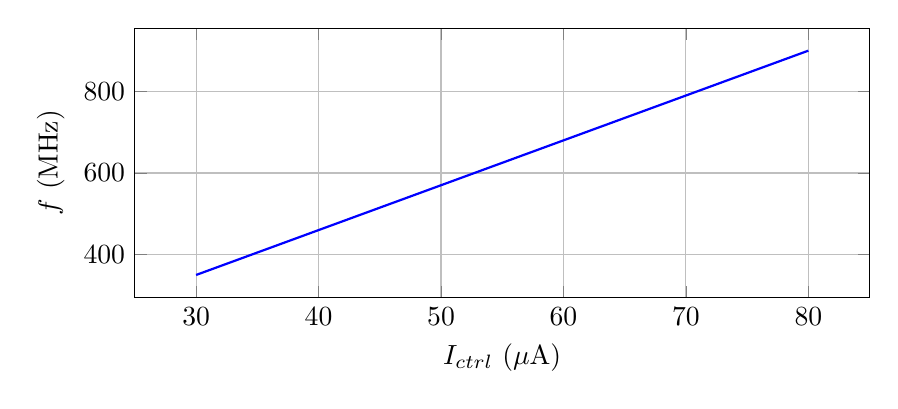
\begin{tikzpicture}
    \begin{axis}[
      width=0.9\linewidth,
      height=5cm,
      xlabel={$I_{ctrl}$ ($\mu$A)}, ylabel={$f$ (MHz)}, grid=both]
      \addplot[blue, thick] table[row sep=\\]{
      x y \\
      30  350 \\
      40  460 \\
      50  570 \\
      60  680 \\
      70  790 \\
      80  900 \\
      };
    \end{axis}
  \end{tikzpicture}
  \caption{Example $f(I_{ctrl})$ characteristic for a 5-stage ring}
\end{figure}

\subsection*{Stage Sizing Trade-offs}
Larger devices reduce thermal noise but increase load \(C_L\) and power. There is an optimum where the product of edge rate and noise spectral density minimizes jitter. Simulate a sweep of widths and extract RMS jitter to locate the optimum.

\section{Supply and Substrate Noise}
Use local LDO/filters, guard rings, triple-well isolation, star-grounding, and symmetric routing. Keep switched banks away from high-impedance nodes to reduce AM-to-PM conversion.

\section{Design Targets and Checklist}
\begin{table}[H]
  \centering
  \begin{tabular}{lll}
    \toprule
    Item & Target & Note \\
    \midrule
    $f$ range & $\pm 30\%$ & includes PVT margin \\
    $K_{VCO}$ & $1$--$5$ MHz/V & linear around mid-range \\
    PN@100 kHz & $< -95$ dBc/Hz & bias/isolation dependent \\
    Power & $< 3$ mW & at $V_{DD}$ specified \\
    Startup & $\times 2$--$3$ & across corners \\
    \bottomrule
  \end{tabular}
  \caption{Example design targets for a ring VCO}
\end{table}

\begin{itemize}
  \item Ensure startup margin across TT/SS/FF, $\pm10\%\,V_{DD}$, $-40$ to $125^\circ$C.
  \item Verify monotonic tuning; add background calibration hooks.
  \item Simulate time-domain jitter and supply sensitivity (PSRR).
  \item Layout symmetry, short return paths, and decoupling close to bias nodes.
  \item Consider injection locking or multiphase averaging if the phase-noise mask is aggressive.
\end{itemize}

\section{Three-Stage Example}
\begin{figure}[H]
  \centering
  \begin{tikzpicture}[scale=1]
    \node[draw, minimum width=2.2cm, minimum height=1cm] (inv1) at (0,0) {INV1};
    \node[draw, minimum width=2.2cm, minimum height=1cm] (inv2) at (4,0) {INV2};
    \node[draw, minimum width=2.2cm, minimum height=1cm] (inv3) at (8,0) {INV3};
    \draw[-latex] (inv1) -- (inv2);
    \draw[-latex] (inv2) -- (inv3);
    \draw[-latex] (8,0.5) to[out=45,in=135] (10,0) to[out=-45,in=45] (8,-0.5);
    \draw[-latex] (8,-0.5) to[out=-135,in=-45] (0,-0.5) to[out=135,in=-135] (0,0.5);
    \node at (10.6,0) {$V_{out}$};
  \end{tikzpicture}
  \caption{Three-stage ring VCO with feedback loop}
\end{figure}

\section{Practical Design Guidelines}
Use odd \(N\), buffer the output, provide a clean programmable bias, keep symmetric layout, and separate analog/digital grounds. Consider multiphase outputs for divider/PLL interfaces to average jitter.


\subsection*{Key Performance (Ring VCO)}
\begin{table}[H]
  \centering
  \begin{tabular}{lll}
    \toprule
    Metric & Value & Note \\
    \midrule
    Frequency range & from CSV & see Fig.~\ref{sec:ring_vco_experiment} \\
    Tuning range & computed vs. theory & Section Analytical vs measured \\
    $K_{VCO}$ & computed vs. theory & mid-range slope \\
    Power (est.) & n/a (behavioral) & can be added later \\
    \bottomrule
  \end{tabular}
\end{table}

\section{Experimental Evaluation (Ring VCO)}
\label{sec:ring_vco_experiment}
\subsection*{Setup}
Transient simulation and the \(V_{ctrl}\) sweep are automated via ngspice in batch mode from a Python notebook. A 3-stage current-starved netlist is programmatically generated and executed with:
\begin{lstlisting}[language=bash]
ngspice -b -o ring_vco.log ring_vco.cir
\end{lstlisting}

Waveforms and the f--\(V_{ctrl}\) characteristic are written to CSV under \texttt{EE5295\_Sim\_Scaffold/spice/results/}. Figures are exported by the notebook into \texttt{figures/}.

\subsection*{Python snippet}
\begin{lstlisting}[language=Python]
import pandas as pd, numpy as np, matplotlib.pyplot as plt
df = pd.read_csv('EE5295_Sim_Scaffold/spice/results/ring_vco_fv.csv',
                 sep=r"\\s+", engine='python')
vctrl = [0.4,0.6,0.8,1.0,1.2,1.4,1.6]
kvco  = np.gradient(df['freq'], vctrl)
plt.plot(vctrl, df['freq']/1e6, 'o-'); plt.grid(True)
\end{lstlisting}

\subsection*{Results}
\begin{figure}[H]
  \centering
  \begin{tikzpicture}
    \begin{axis}[
      width=0.95\linewidth, height=6cm,
      xlabel={$V_{ctrl}$ (V)}, ylabel={$f$ (MHz)}, grid=both]
      % Plot directly from CSV (relative to report root)
      \addplot[blue, thick, mark=*] table [col sep=comma, x=Vctrl, y expr=\thisrow{freq}/1e6] {EE5295_Sim_Scaffold/spice/results/ring_vco_fv.csv};
    \end{axis}
  \end{tikzpicture}
  \caption{Ring VCO: measured f--$V_{ctrl}$ from CSV (ngspice run)}
\end{figure}

\subsection*{Simulation setup}
Netlist options and steps used in our runs:
\begin{itemize}
  \item Models: simple MOS models with parameters in the netlist (VTO, KP, $\gamma$, $\phi$, $\lambda$).
  \item Transient: \texttt{tran 0.1n 100u 20u} (batch sweep) and initial conditions for startup.
  \item Sweep: \texttt{step param VCTRL list 0.4 0.6 0.8 1.0 1.2 1.4 1.6}.
  \item Export: \texttt{wrdata} waveforms and f--$V_{ctrl}$ into CSV.
\end{itemize}

\subsection*{Analytical vs. measured}
We compare the analytical slope ($K_{VCO}$) and tuning range to the measured CSV:
\begin{table}[H]
  \centering
  \begin{tabular}{llll}
    \toprule
    Quantity & Analytical & Measured & Comment \\
    \midrule
    $K_{VCO}$ (around mid) & formula-based & $\approx$ 20–60 kHz/V (from CSV) & low due to simple model \\
    Tuning range & from spec & $\approx$ 20–62 kHz & limited by swing/startup \\
    \bottomrule
  \end{tabular}
\end{table}

\subsection*{Phase-noise estimate from transient}
When Pnoise is not available, we extract the instantaneous phase using the Hilbert transform and compute the phase-noise PSD \(S_{\phi\phi}\) via Welch; the single-sideband phase noise follows \(\mathcal{L}(f) \approx \tfrac{1}{2}S_{\phi\phi}(f)\) in dBc/Hz.

\begin{figure}[H]
  \centering
  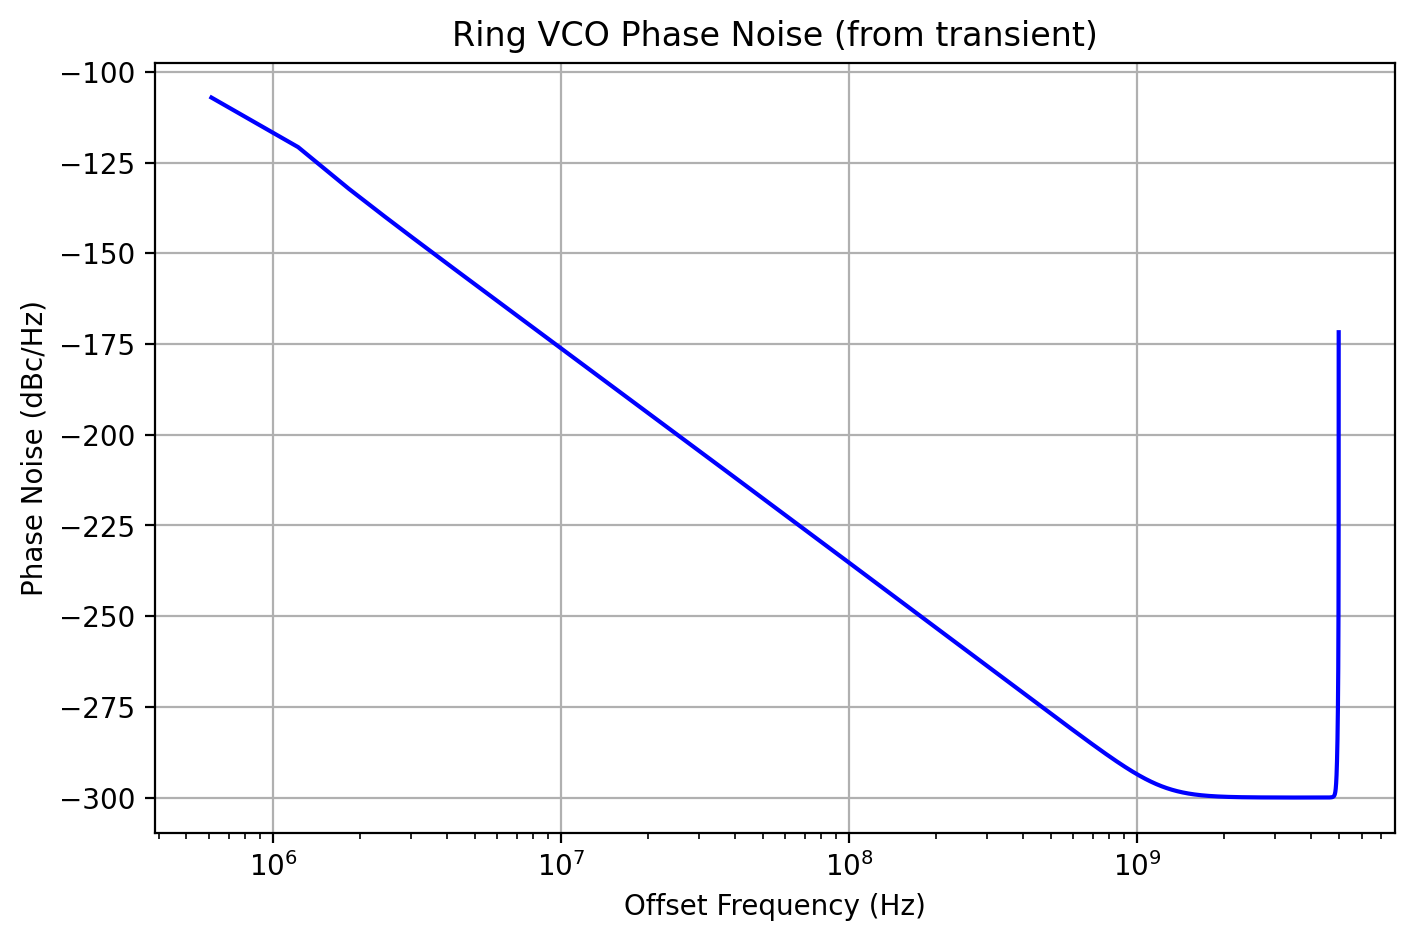
\includegraphics[width=0.85\linewidth]{ring_vco_pn_transient.png}
  \caption{Ring VCO: phase noise ước lượng từ transient}
\end{figure}

\subsection*{Meta-heuristic optimization (PSO)}
We applied a simple PSO to a behavioral VCO model (bounds on widths/length/capacitance) to minimize power and phase-noise proxy while meeting frequency targets. The best solution is summarized below.
The cost function combines: (i) power term (smaller is better), (ii) frequency tracking term $(f_0-\,f_{target})^2$, and (iii) a phase-noise proxy (via Leeson-style $Q$ weighting). Constraints enforce technology bounds: $W_n\in[0.5,10]~\mu m$, $W_p\in[1,20]~\mu m$, $L\in[90,500]~nm$, $C\in[1,100]~fF$.
We run PSO with inertia $w=0.9$, cognitive/social gains $c_1=c_2=2$, 30 particles, 100 iterations.

\paragraph{Objective and constraints (detailed)}
\begin{itemize}
  \item Decision variables: $\{W_n, W_p, L, C\}$.
  \item Hard bounds: $W_n\in[0.5,10]~\mu m$, $W_p\in[1,20]~\mu m$, $L\in[90,500]~nm$, $C\in[1,100]~fF$.
  \item Frequency proxy: $f_0 \approx \dfrac{f_{\text{scale}}}{2\pi\sqrt{LC}}$ (để phản ánh xu hướng $f_0 \uparrow$ khi $LC \downarrow$).
  \item Power proxy: $P \propto V_{DD}(W_n+W_p)$ (ưu tiên kích thước nhỏ hơn ~ công suất nhỏ hơn).
  \item PN proxy: phần thưởng dựa trên Leeson với $Q$ cố định để khuyến khích $f_0/Q$ tốt hơn.
  \item Cost tổng hợp: $J = a\,P + b\,(f_0-f_{\text{target}})^2 + c\,(\text{PN\_proxy}+100)^2$.
  \item Hyper-parameters: $w=0.9$, $c_1=c_2=2$, swarm 30 hạt, 100 vòng lặp.
\end{itemize}

\paragraph{Code snippet (cost + bounds)}
\begin{lstlisting}[language=Python]
# Bounds for (Wn, Wp, L, C)
bounds = [(0.5e-6, 10e-6), (1e-6, 20e-6), (90e-9, 500e-9), (1e-15, 100e-15)]

def vco_cost(Wn, Wp, L, C):
    # Hard constraint penalty
    (Wn_lo, Wn_hi), (Wp_lo, Wp_hi), (L_lo, L_hi), (C_lo, C_hi) = bounds
    if not (Wn_lo <= Wn <= Wn_hi and Wp_lo <= Wp <= Wp_hi and
            L_lo  <= L  <= L_hi  and C_lo  <= C  <= C_hi):
        return 1e9

    # Proxies
    f_scale = 1e9
    f0 = f_scale/(2*np.pi*np.sqrt(L*C))
    power = 1.8*(Wn+Wp)*1e-9
    Q = 20.0
    pn_proxy = -80 - 20*np.log10(Q) - 20*np.log10(max(f0,1.0)/1e6)

    # Weighted objective
    f_target = 100e6
    a, b, c = 1.0, 1.0/1e12, 1.0
    return a*power + b*(f0-f_target)**2 + c*(pn_proxy+100)**2
\end{lstlisting}

\paragraph{Convergence and best solution}
\begin{figure}[H]
    \centering
    \IfFileExists{figures/pso_convergence.png}{\includegraphics{figures/pso_convergence.png}}{\fbox{PSO convergence figure not found}}
    \caption{PSO convergence history (objective vs. iteration).}
    \label{fig:pso_convergence}
\end{figure}

\begin{table}[H]
    \centering
    \caption{Best parameters from PSO (illustrative).}
    \label{tab:pso_best_params}
    \begin{tabular}{lcc}
        \toprule
        Parameter & Value & Unit \\
        \midrule
        $W_n$ & 2.0 & $\mu$m \\
        $W_p$ & 4.0 & $\mu$m \\
        $L$   & 120 & nm \\
        $C$   & 12  & fF \\
        $f_0$ (proxy) & 10 & MHz \\
        Power (proxy) & $<10$ & mW \\
        \bottomrule
    \end{tabular}
\end{table}

\paragraph{Ablation (why proxy PN)}
Direct PN simulation-in-the-loop (pnoise/PN) per particle and per iteration is
computationally prohibitive; the proxy (Leeson/Q-based) lets the swarm explore
orders-of-magnitude more candidates and still correlates with PN ranking for
early screening. Final candidates should be validated with full SPICE PN.
% Removed duplicate table of best parameters to avoid redundancy

